\section{Background}
In this section, we cover the background subjects needed to formally pose the problem and solutions 
in this thesis.  We start with two types of combinatorial structures, linkages and polygonal 
linkages.  We then discuss the configuration spaces of linkages and polygonal linkages.   We then 
look into an alternate representation of linkages, disk arrangements and state the disk arrangement 
theorem but do not show its proof.  We then look at satisfiability problems, a logic engine that 
encodes a type of satisfiability problems.  Finally, we cover the basic definitions of algorithm 
complexity for $\textbf{P}$ and $\textbf{NP}$
\subsection{Linkages}
%graph -> G = (V,E)
%linkage -> (G,l)
%embedding -> 
There are two parts to a linkage, the graph and the edge length mapping.   A \textit{graph} is an 
ordered pair $G = (V,E)$ comprising of a set $V$ of vertices or together with a set $E$ of edges or 
lines.  For every edge $e \in E$, there is a distinct pair of vertices in $V$ that it represents, 
$(u,v) \in E$.  While graphs can have vertices that may not correspond to any edges, we rule out 
this possibility for linkages.  The edge length assignement mapping of a linkage is $l: E \mapsto 
\bbr^+$. A linkage is still an abstract combinatorial structure until an \textit{embedding} on the 
graph of the linkage is posed, i.e. $\Pi : V \mapsto \bbR^{2}$. $\Pi$ has the \textit{proper 
embedding} property, if for every edge $(u,v) \in E$ such that $l\left( \left(u,v\right) \right) 
= \left\vert \Pi(u) - \Pi(v) \right\vert$ is true. The \textit{realization} of the the linkage is 
said to be the range $\Pi$, i.e. $\Pi(V)$.  Without loss of generality, for this paper, we focus on 
linkages that have simple planar graph properties, i.e.:
\begin{itemize}
\item[\rn{1}] does not have edges that cross,
\item[\rn{2}] does not have loops, i.e. $(v,v) \in E$, or
\item[\rn{3}] does not have multiple edges between any pair of vertices.
\end{itemize}  
We may visit special cases in which we look at planar graphs that satisfy the last two conditions 
but not the first, e.g.:
%graph component of the linkage   the plane.  A linkage 
%\textit{embedding} is $L : V \mapsto 
%\bbR^{2}$.
% A \textit{linkage} is an ordered pair $G = (V,E)$ comprising of a set $V$ of vertices or nodes 
% together with a set $E$ of edges or lines. This definition is commonly used for graphs.  Mapping 
% the linkage $G$ into the plane is said to be the \textit{embedding}, i.e. $L : V \mapsto 
% \bbR^{2}$.  A length function correspond to a linkage, $l: E \mapsto \bbr^+$ gives a length to an 
% edge in the linkage.  If We consider a \textit{realization} of a linkage is range of $L$, i.e. 
% $L(V)$. If for every edge $(u,v) \in E$ such that $l\left( \left(u,v\right) \right) = \left\vert 
% L(u) - L(v) \right\vert$ is true, then $L$ is said to be a \textit{proper embedding} of $G$.
\begin{figure}[h]
\begin{center}
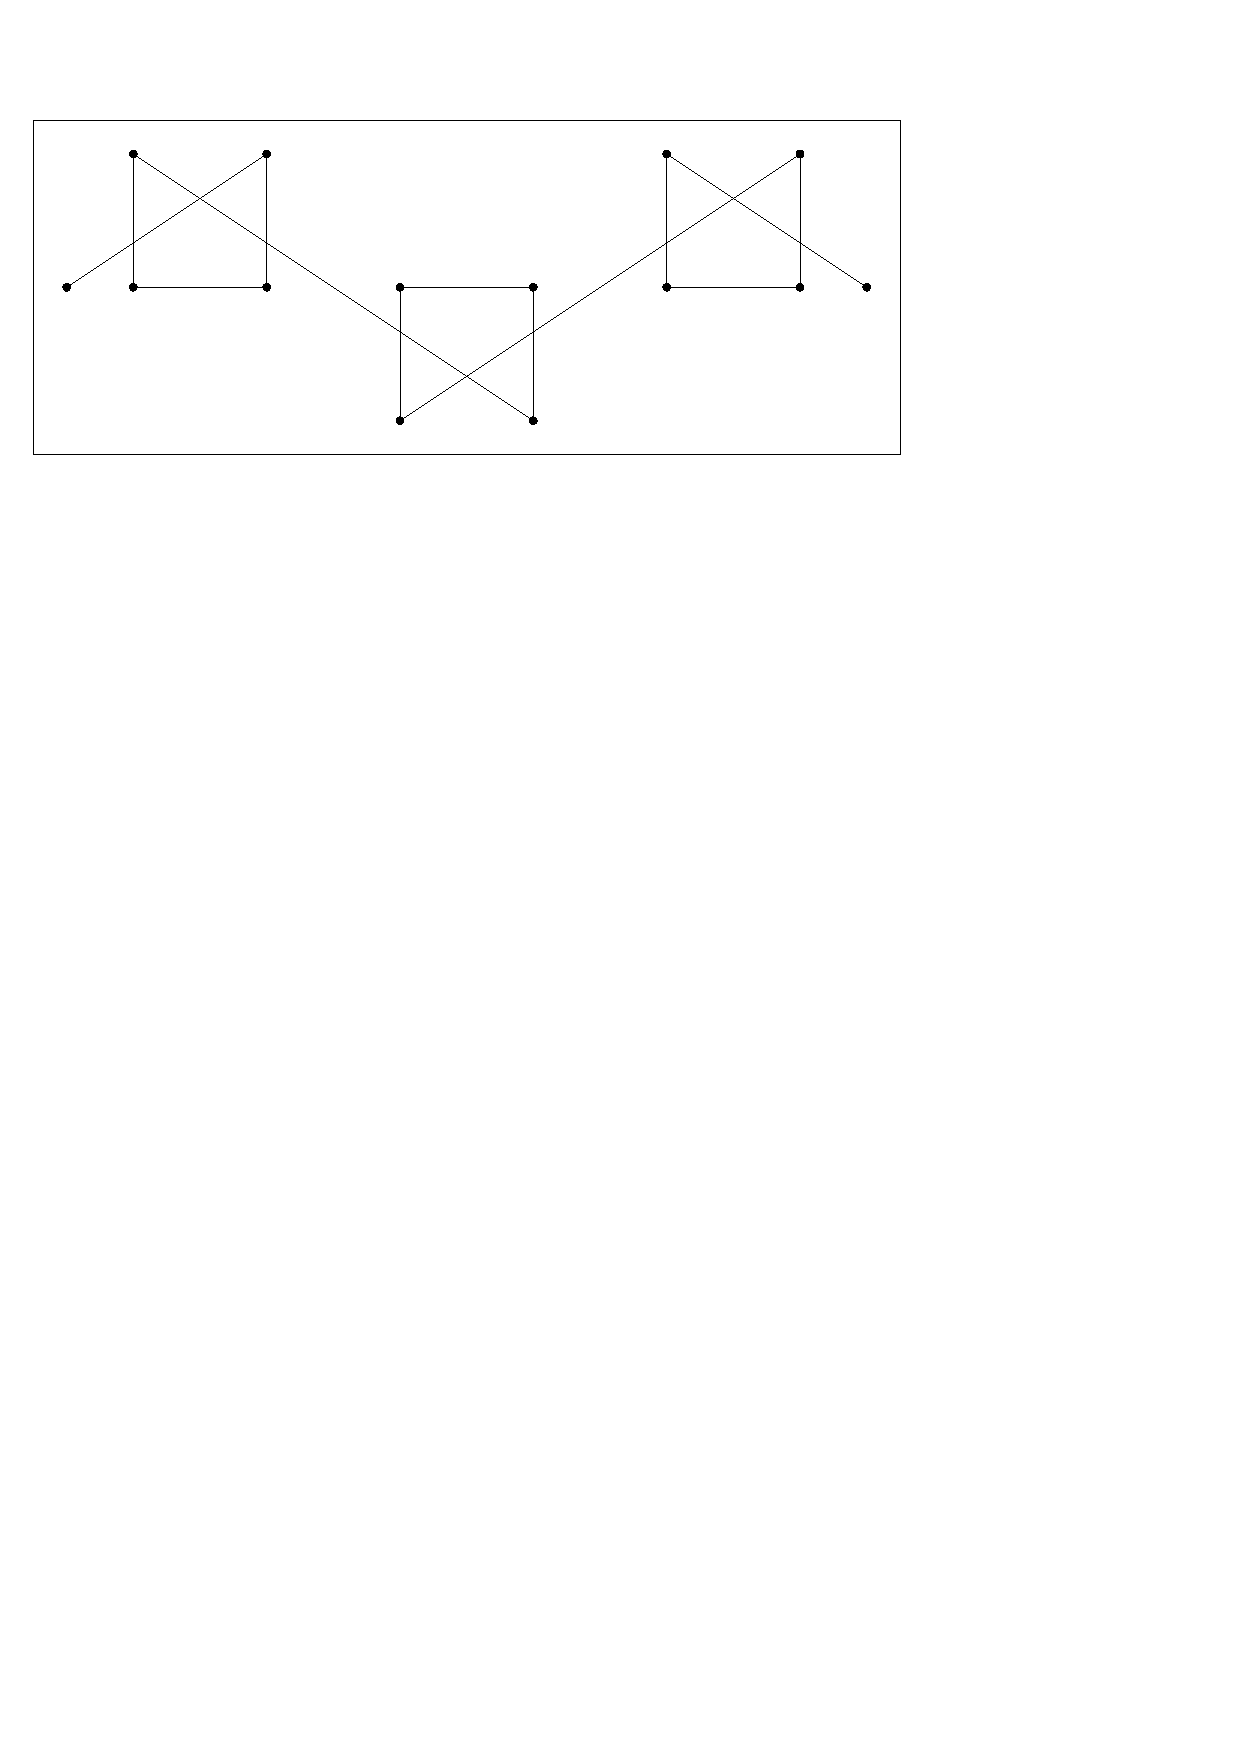
\includegraphics[scale=1]{graphics/crossingEdgeLinkage.pdf}
\end{center} 
\caption{A linkage where edges cross however it does not contain loops or multiple edges between 
vertices.}
\label{fig:linkage-3}
\end{figure}
\subsection{Polygonal Linkages}
\begin{figure}[h]
\begin{center}

\includegraphics[scale=1]{graphics/hingeOnThreeDistinctPolygons.pdf}
\end{center} 
\caption{(a) A polygonal linkage with a non-convex polygon and two hinge points corresponding to 
three polygons.  Note that hinge points correspond to two distinct polygons.(b) Illustrating that 
two hinge points can correspond to the same boundary point of a polygon.}
\label{fig:linkage-1}
\end{figure}
%describe how it is a generalization of Linkages.
Polygonal linkages have some differences to linkages.  Polygonal linkages have a combinatorial 
structure that is graph-like.  A polyonal linkage's combinatorial structure is an ordered pair 
$\left(\HH,\PP \right)$.  Instead of a set of vertices, there is a set of hinges, $\HH$;  instead 
of a set of edges, there is a set of polygons, $\PP$. Formally, a \textit{hinge} $h\in \HH$ 
corresponds to two points on the boundary of two distinct polygons in $\PP$.  Since polygons do not 
exhibit a length property, a polygonal linkage does not have an edge length mapping.  


Polygon linkages are similar to linkages.  They are an ordered pair of sets, with the exception 
that the set of vertices become a set of hinges, $\HH$, and the set of edges become a set of 
polygons, $\PP$.  Formally, a \textit{polygonal linkage} is an ordered pair, $G = (\HH,\PP)$,  
comprises of a set of polygons, $\PP$, and a set of hinge points $\HH$ where each hinge $h \in \HH$ 
corresponds to two points on the boundary of two distinct polygons in $\PP$. Mapping the linkage 
$G$ into the plane is said to be the \textit{embedding}, i.e. $L : \HH \mapsto \bbR^{2}$.  We 
consider a \textit{realization} of a polygonal linkage is range of $L$, i.e. $l(\HH)$.

In figure (\ref{fig:linkage-1}), we illustrate that two hinge points can reside on the same point 
in the plane. Figure (\ref{fig:linkage-1}) and figure (\ref{fig:linkage-3}) are examples of special 
cases that we may run into, but do not want to focus heavily on.  They are presented to the reader 
to facilitate understanding of the definitions of polygonal linkages and linkages respectively.  
Without loss of generality, for this paper, we focus on polygonal linkages that are 
equivalent to simple planar graphs.
%Foigr each hinge point $h \in \HH$, there 
%exists some subset $P \subset \PP$ with 
%at least cardinality of 2 such that for each polygon $p \in P$, $h$ corresponds to some point on 
%the boundary of $p$.  When the polygonal linkage is embedded in the plane, the hinge point is 
%where 
%the polygons of $P$ \it{kiss}.  
% show an example of polygonal linkages
\begin{figure}[h]
\begin{center}
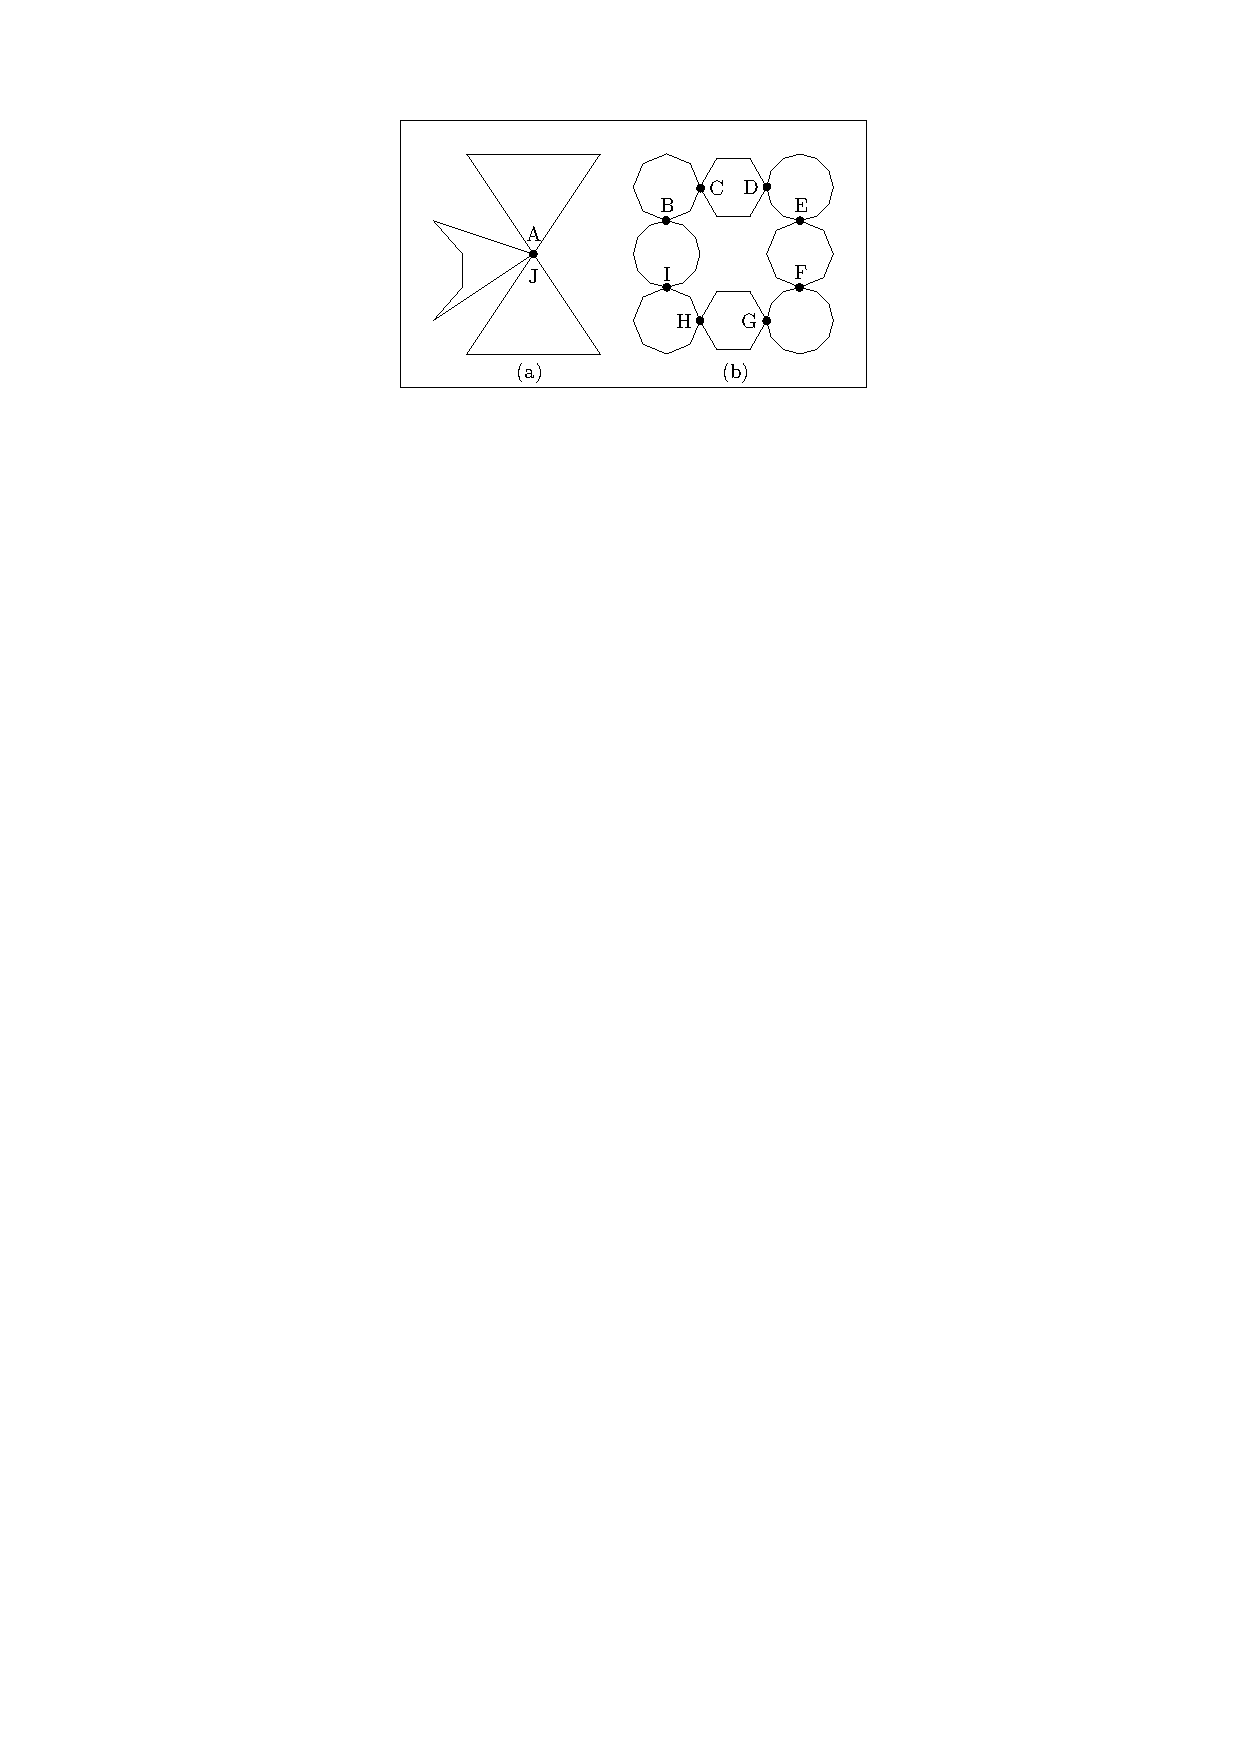
\includegraphics[scale=1]{graphics/PolygonalLinkageExamples.pdf}
\end{center} 
\caption{(a) A polygonal linkage with a non-convex polygon and a hinge point corresponding to three 
polygons.  (b) A polygonal linkage with 8 regular polygons.}
\label{fig:linkage-2}
\end{figure}
For the remainder of this thesis, we'll focus on the polygonal linkages with the following 
restrictions:
\begin{enumerate}
 \item  For each hinge point $h \in \HH$, there exists some subset $P \subset \PP$ with 
exactly cardinality of 2, and
\item every polygon in $\PP$ is convex.
\end{enumerate}
Formally, we define a \it{polygonal linkage} as an ordered pair $L = (\HH,\PP)$ comprising of a 
set of hinges, $\HH$, where each hinge $h\in \HH$ corresponds to two points on the boundary of two 
distinct polygons. A \emph{realization} of a polygonal linkage is an interior-disjoint placement of 
congruent copies of the polygons in $\PP$ such that the points corresponding to each hinge are 
identified (Fig. \ref{fig:1}). 
\subsection{Properties of Linkages and Graphs}
%things to do:
%1) Isomorphism -> graph property
%2) Ordered graph -> graph property ultimately for polygonal linkages.  
%To describe the types of motion that we are interested in linkages we must define the graph 
%isomorphism.  
Given two graphs $G=(V_1,E_1)$ and $G_2 = (V_2,E_2) $, a bijection $f: V_1 \mapsto 
V_2$ 
such that for any two vertices $u,v \in V_1$ that are adjacent, i.e. $(u, v) \in E_1$, if and only 
if $(f(u),f(v)) \in E_2$. 
\begin{table}[!ht]
\begin{center}
$$\begin{array}{|c|c|c|}\hline
\text{Graph}&\text{Vertices}&\text{Edges}\\\hline
G_1&\left\lbrace a,b,c,d,e \right\rbrace & \left\lbrace (a,b),(b,c),(c,d),(d,e),(e,a) \right\rbrace 
\\\hline
G_2&\left\lbrace 1,2,3,4,5 \right\rbrace & \left\lbrace (1,2),(2,3),(3,4),(4,5),(5,1) \right\rbrace 
\\\hline
\end{array} $$
\caption{Two graphs that are isomorphic with the alphabetical isomorphism $f(a)=1$, $f(b)=2$, $f(c) 
= 3$, $f(d)=4$, $f(e)=5$.}
\end{center} 
\label{table:linkages-1}
\end{table} 
% show an example of polygonal linkages
\begin{figure}[!h]
\begin{center}
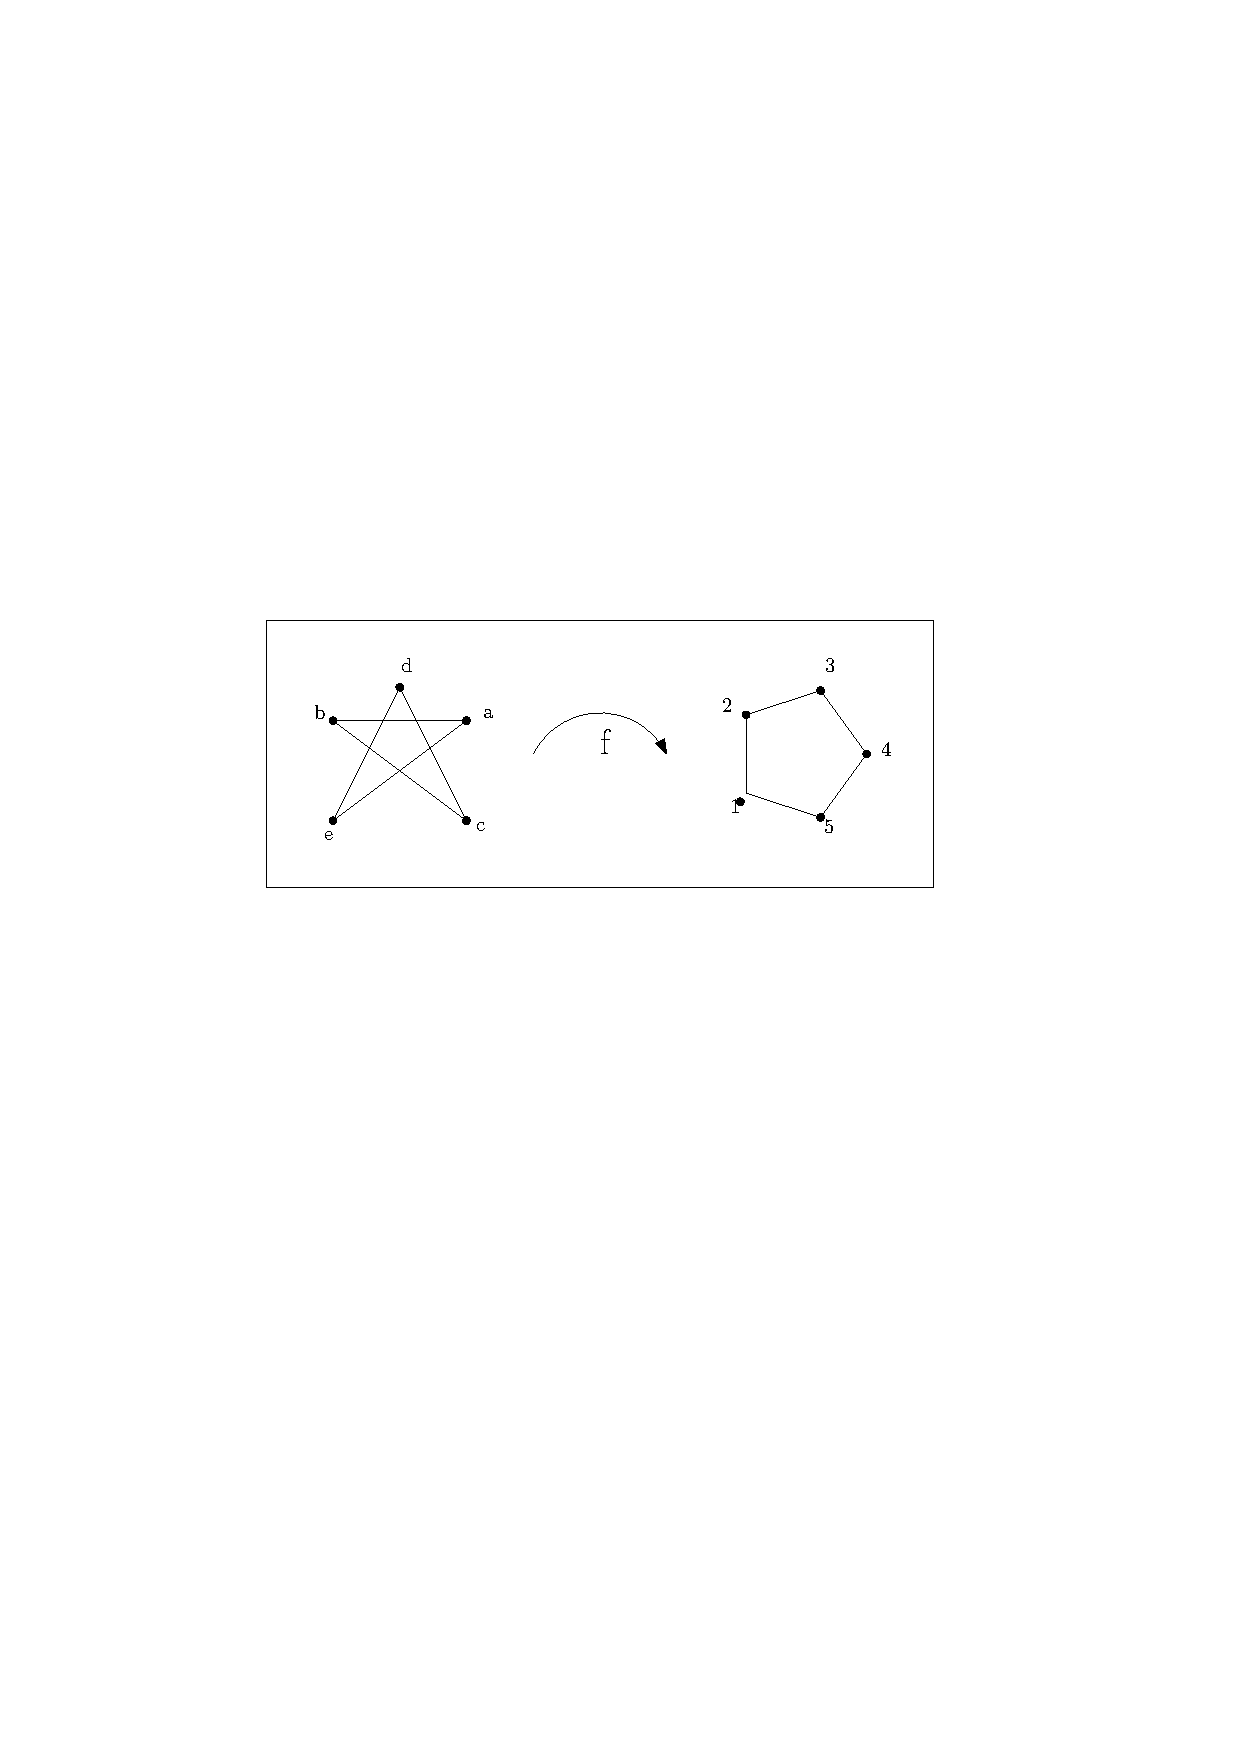
\includegraphics[scale=1]{graphics/graphIsomorphismExample.pdf}
\end{center} 
\caption{This figure depicts the graph isomorphism shown in Table 
(\ref{table:linkages-1}) between 
$V_1$ and $V_2$ in the plane.}
\label{fig:configuration-3}
\end{figure}
Next we add restrictions to our graph isomorphisms to narrow our focus:
\begin{itemize}
\item[\rn{1}] We focus on isomorphisms for planar graphs and or polygonal linkages, simple planar 
graphs, and
\item[\rn{2}] the isomorphism preserves edge lengths (polygonal area), e.g. $d(u,v) = d(f(u),f(v))$.
\end{itemize}  
With these restrictions of our isomorphisms, we can begin to describe a range of motion to 
transform a linkage.  That range of motion is said to be the configuration space of that linkage.  
To expand on this concept, for given linkage, $L=(V,E)$, and for a given vertex $v \in V$, the set 
of points in which $v$ can be realized in the plane would be the configuration space for that 
vertex, $C_v$.  Defining some order of the vertices in $L$, i.e. $V = \left\lbrace v_n 
\right\rbrace_{i=1}^n$, then the \it{configuration space} for $L$ is said to be the cartesion 
product of the configuration space of vertices:
\subsection{Summary}
\begin{table}[!ht]
\begin{center}
$$\begin{array}{|l|c|c|}
 \hline
&\text{Linkages}&\text{Polygonal Linkages}\\\hline
\text{Ordered Pair}&G&G\\\hline
\text{Edges}&E&\HH\\\hline
\text{Vertices}&V&\PP\\\hline
l&l&\text{N.A.}\\\hline
\text{Embedding of }G&\Pi : V \mapsto \bbr^2&\PP ' = \left\lbrace P_i ' 
\right\rbrace_{i=1}^n\\\hline
\text{Realization}&\text{See (a)}&\text{See (b)}\\\hline
\end{array}
\caption
$$
\caption{(a)The realization for a linkage is for any edge $(u,v) \in E$ such that $\left\vert 
\Pi(u)-\Pi(v)\right\vert = l(u,v)$.(b)A \emph{realization} of a polygonal linkage is an 
interior-disjoint placement of congruent copies of the polygons in $\PP$ such that the points 
corresponding to each hinge are identified (Fig. \ref{fig:1}, left).(c).}
\end{center} 
\label{table:linkages-2}
\end{table} 
%1) 
%DESCRIBE THE FOLLOWING:
%1)CONFIGURATION SPACE AS A VECTOR SPACE OF DIMENSION 2^N WHERE EDGE LENGTH IS PRESERVED.
%2)PINNING 1 VERTEX TO ORIGIN AND A NEIGHBOR, ADD MOTIVATION TO PREVENT ROTATION AND TRANSLATIONS.

% \begin{equation}\label{eqn:linkages-1}
% C(L) = C_{v_1} \cross C_{v_2} \cross \cdots \cross C_{v_n}
% \end{equation} 
% Some food for thought on configuration spaces and motions on linkages:
% \begin{itemize}
% \item[\rn{1}] A configuration space is said to be \it{connected} if there is a continuous mapping for any two planar realizations (linkages) of a graph in the plane.  Otherwise it is said to be \it{disconnected}.
% \item[\rn{2}] If the configuration space of a vertex, $C_v$, is a singleton set, then the vertex is said to be \it{pinned}. Otherwise it is said to be \it{free}.
% \item[\rn{3}] The types of motions (mappings) that we refrain from using on linkages are translations.
% \end{itemize}
% Note that configuration spaces for polygonal linkages are described similarly.
% \subsubsection{Realizability of Linkages}
% Suppose we had two configurations of a linkage, $\mathcal{A}$ and $\mathcal{B}$.  A question that can be posed is can we reconfigure $\mathcal{A}$ to $\mathcal{B}$ continuously while respecting simple planar graph conditions?  The answer to this question is a yes or no.  If yes, then there must exist a path connected configuration space between $\mathcal{A}$ and $\mathcal{B}$.  It has been shown that this problem can be posed as a planar satisfiability problem \cite{Breu19983,mulzer2008minimum} (Later on in this paper we'll cover satisfiability problems).  This is the type of problem that we face in this paper.  We will continue to explore this in a different manner, with circle packings.
\newpage 
